\subsection{Iterazioni di punto fisso}

\begin{examplebox}[: esempio di introduzione]
    Con una calcolatrice si può facilmente verificare che applicando ripetutamente la funzione $\cos$ partendo dal numero $1$ si genera la seguente successione di numeri reali:
    \begin{equation*}
        \begin{array}{lclcl}
            x^{\left(1\right)}  &=& \cos\left(1\right)                  &=& 0.54030230586814 \\ [1em]
            x^{\left(2\right)}  &=& \cos\left(x^{\left(1\right)}\right) &=& 0.85755321584639 \\
            \vdots              & &                                     & & \\
            x^{\left(10\right)} &=& \cos\left(x^{\left(9\right)}\right) &=& 0.74423735490056 \\
            \vdots              & &                                     & & \\
            x^{\left(20\right)} &=& \cos\left(x^{\left(19\right)}\right)&=& 0.73918439977149
        \end{array}
    \end{equation*}
    Che tende al valore $\alpha = 0.73908513$.
\end{examplebox}

\noindent
Con l'esempio di introduzione è possibile capire il punto fisso. Essendo per costruzione $x^{\left(k+1\right)} = \cos\left(x^{\left(k\right)}\right)$ per $k = 0, 1, \dots$ (con $x^{\left(0\right)} = 1$), $\alpha$ è tale che $\cos\left(\alpha\right) = \alpha$. Quindi, $\alpha$ viene detto punto fisso della funzione coseno.

\highspace
\begin{flushleft}
    \textcolor{Green3}{\faIcon{question-circle} \textbf{Perché è interessante?}}
\end{flushleft}
Se $\alpha$ è un punto fisso per il coseno, allora esso è uno zero della funzione $f\left(x\right) = x - \cos\left(x\right)$ ed il metodo appena proposto potrebbe essere usato per il calcolo degli zeri di $f$.

\highspace
\begin{flushleft}
    \textcolor{Red2}{\faIcon{exclamation-triangle} \textbf{Non tutte le funzioni hanno un punto fisso}}
\end{flushleft}
Non tutte le funzioni ammettono punti fissi. Ad esempio, ripetendo l'esperimento dell'esempio con una funzione esponenziale a partire da $x^{\left(0\right)} = 1$, dopo soli 4 passi si giunge ad una situazione di \emph{overflow} (figura \ref{fig: non tutte le funzioni hanno un punto fisso}, pagina \pageref{fig: non tutte le funzioni hanno un punto fisso}).

\begin{definitionbox}
    Data una funzione $\phi: \left[a, b\right] \rightarrow \mathbb{R}$, trovare $\alpha \in \left[a,b\right]$ tale che:
    \begin{equation*}
        \alpha = \phi\left(\alpha\right)
    \end{equation*}
    Se tale $\alpha$ esiste, viene detto un \definition{punto fisso} di $\phi$ e lo si può determinare come limite della seguente successione:
    \begin{equation}\label{eq: successione punto fisso}
        x^{\left(k+1\right)} = \phi\left(x^{\left(k\right)}\right) \hspace{2em} k \ge 0
    \end{equation}
    Dove $x^{\left(0\right)}$ è un dato iniziale. L'algoritmo viene chiamato \definition{iterazioni di punto fisso} e la funzione $\phi$ è detta \definition{funzione di iterazione}.
\end{definitionbox}

\noindent
Dalla definizione, si deduce che l'esempio introduttivo è un algoritmo di iterazioni di punto fisso per la funzione $\phi\left(x\right) = \cos\left(x\right)$.

\newpage

\begin{figure}[!htp]
    \centering
    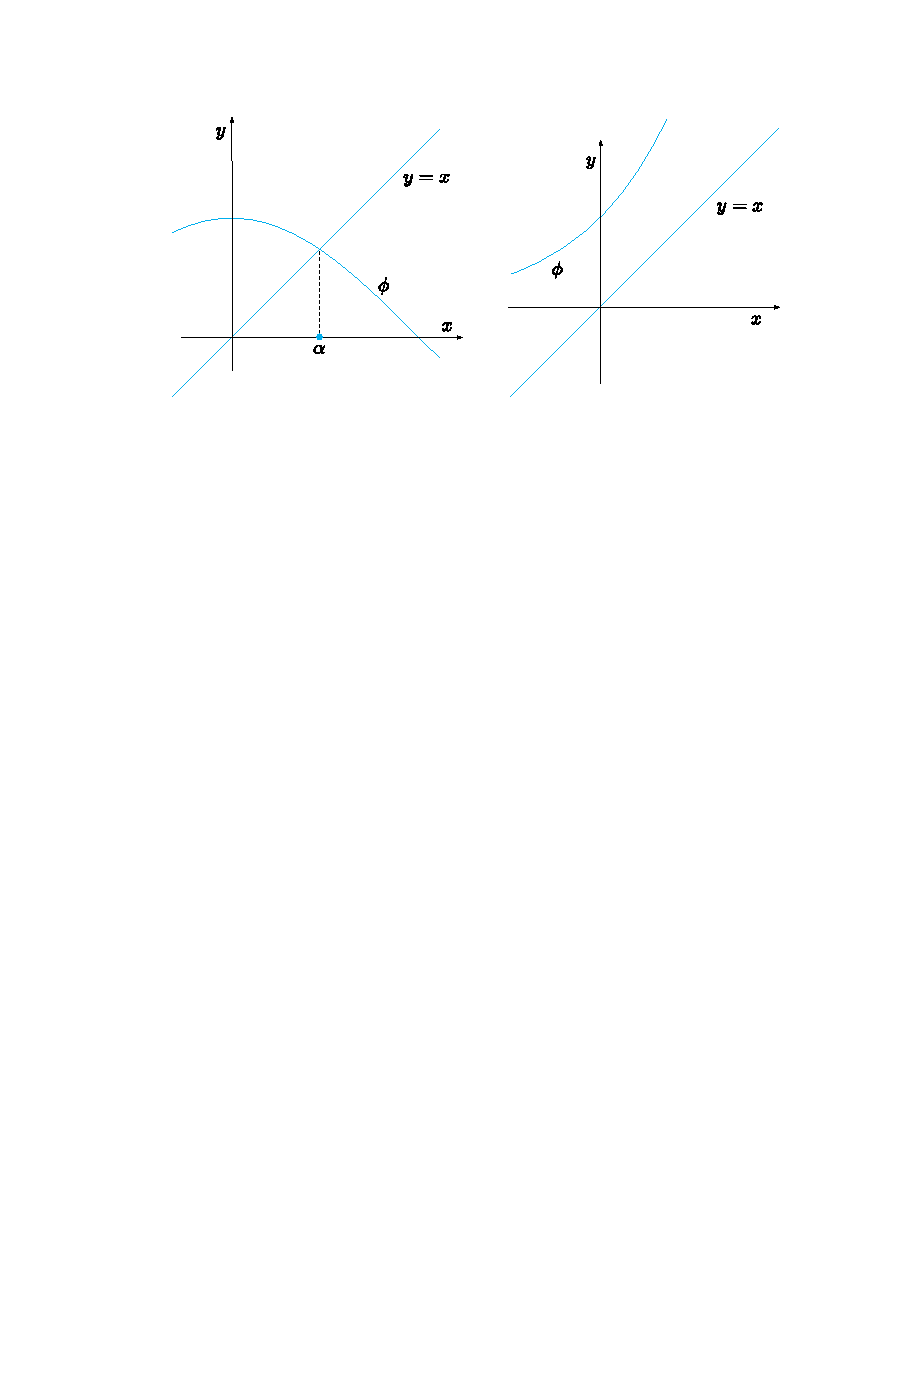
\includegraphics[width=\textwidth]{img/iterazioni-di-punto-fisso-1.pdf}
    \caption{La funzione $\phi\left(x\right) = \cos\left(x\right)$ (sx) ammette un solo punto fisso, mentre la funzione $\phi\left(x\right) = e^{x}$ (dx) non ne ammette alcuno.}
    \label{fig: non tutte le funzioni hanno un punto fisso}
\end{figure}

\hfill

\begin{figure}[!htp]
    \centering
    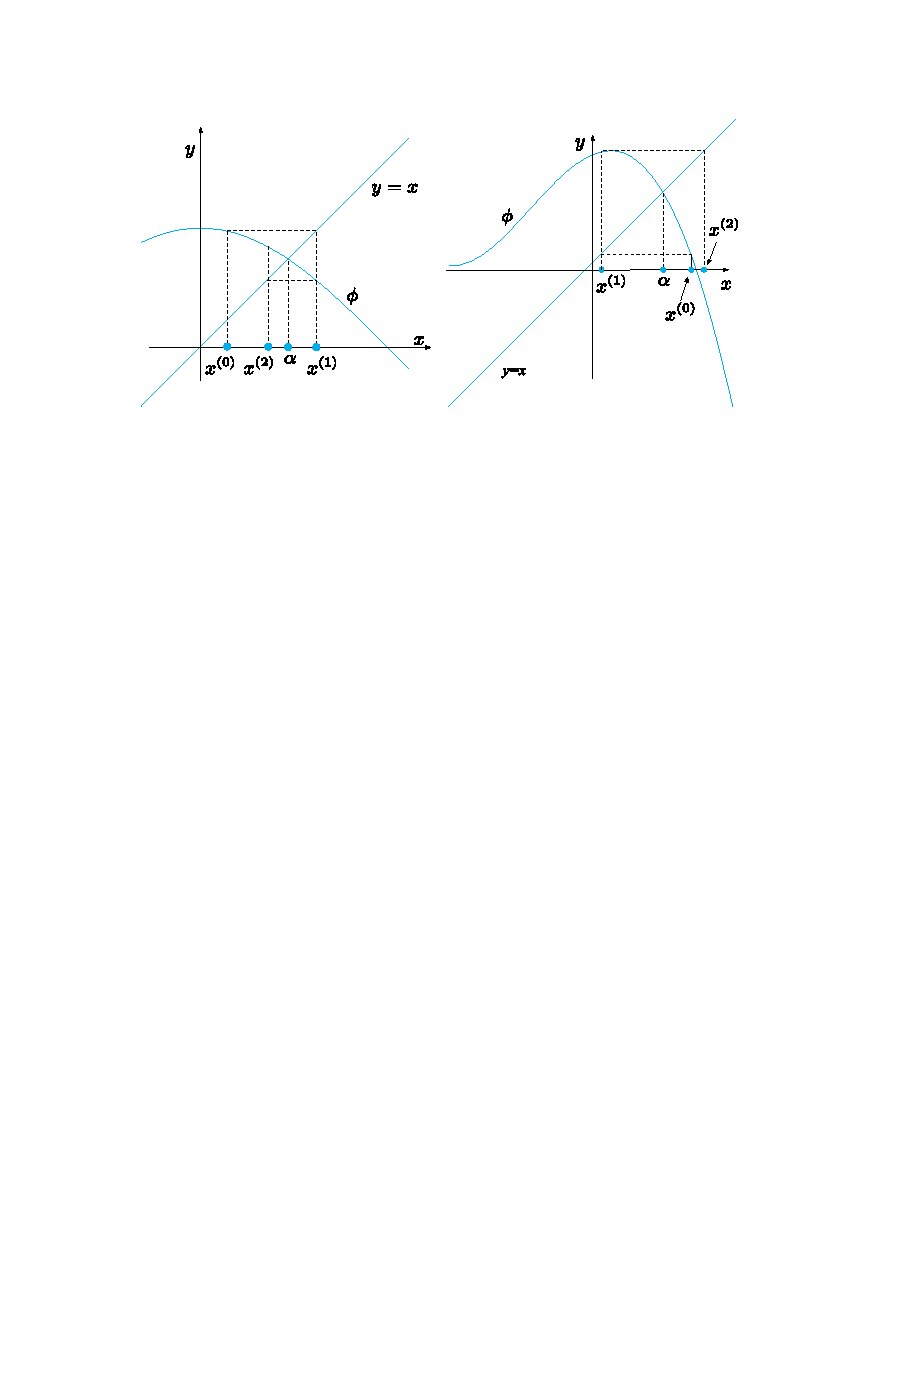
\includegraphics[width=\textwidth]{img/iterazioni-di-punto-fisso-2.pdf}
    \caption{Rappresentazione delle prime iterazioni di punto fisso per due funzioni di iterazione. Le iterazioni convergono verso il punto fisso $\alpha$ (sx), mentre si allontanano da $\alpha$ (dx).}
    \label{fig: interpretazione geometrica di un punto fisso}
\end{figure}

\newpage

\begin{definitionbox}[: quando una funzione ha un punto fisso?]
    Si consideri la successione (formula) \ref{eq: successione punto fisso} a pagina \pageref{eq: successione punto fisso}.
    \begin{enumerate}
        \item Si supponga che $\phi\left(x\right)$ sia continua nell'intervallo $\left[a,b\right]$ e che $\phi\left(x\right) \in \left[a,b\right]$ per ogni $x \in \left[a,b\right]$; allora \textbf{esiste almeno un punto fisso} $\alpha \in \left[a,b\right]$.

        \item Si supponga inoltre che esista un valore $L$ minore di $1$ tale per cui:
        \begin{equation*}
            \left|\phi\left(x_{1}\right)-\phi\left(x_{2}\right)\right| \le L \left|x_{1}-x_{2}\right|
        \end{equation*}
        Per ogni $x_{1},x_{2}$ appartenente all'insieme $\left[a,b\right]$. Con tale supposizione, allora $\phi$ ha un \textbf{unico punto fisso} $\phi\in\left[a,b\right]$ e la successione definita nell'equazione \ref{eq: successione punto fisso} a pagina \pageref{eq: successione punto fisso} converge a $\alpha$, qualunque sia il dato iniziale $x^{\left(0\right)}$ in $\left[a,b\right]$.

        La supposizione scritta in precedenza può essere riassunta in un'equazione:
        \begin{equation}
            \exists L < 1 \:\: t.c. \:\: \left| \phi\left(x_{1}\right)-\phi\left(x_{2}\right)\right| \le L \left|x_{1}-x_{2}\right| \hspace{1em} \forall x_{1},x_{2} \in \left[a,b\right]
        \end{equation}
    \end{enumerate}
\end{definitionbox}

\noindent
Nella pratica è però spesso \textbf{difficile delimitare a priori l'ampiezza dell'intervallo} $\left[a,b\right]$; in tal caso è utile il seguente risultato di convergenza locale:
\begin{theorem}[di Ostrowski]\index{teorema di Ostrowski}\label{theorem: teorema di Ostrowski}
    Sia $\alpha$ un punto fisso di una funzione $\phi$ continua e derivabile con continuità in un opportuno intorno $\mathcal{J}$ di $\alpha$. Se risulta $\left|\phi'\left(\alpha\right)\right| < 1$, allora esiste un $\delta > 0$ in corrispondenza del quale la successione $\left\{x^{\left(k\right)}\right\}$ converge ad $\alpha$, per ogni $x^{\left(0\right)}$ tale che $\left|x^{\left(0\right)} - \alpha \right| < \delta$. Inoltre si ha:
    \begin{equation}
        \displaystyle\lim_{k \rightarrow \infty} \dfrac{
            x^{\left(k+1\right)} - \alpha
        }{
            x^{\left(k\right)}-\alpha
        } = \phi'\left(\alpha\right)
    \end{equation}
\end{theorem}

\highspace
Dal teorema si deduce che le iterazioni di punto fisso convergono almeno linearmente cioè che, per $k$ sufficientemente grande, l'errore del passo $k+1$ si comporta come l'errore al passo $k$ moltiplicato per una costante, $\phi'\left(\alpha\right)$ nel teorema, indipendente da $k$ ed il cui valore assoluto è minore di $1$. Per questo motivo la costante viene chiamata \definition{fattore di convergenza} e la convergenza sarà tanto più rapida quanto più piccola è tale costante.

\begin{definitionbox}[: quando il metodo di punto fisso è convergente]
    Si suppongano valide le ipotesi del teorema di Ostrowski \ref{theorem: teorema di Ostrowski}. Se, inoltre, $\phi$ è derivabile con continuità due volte e se:
    \begin{equation*}
        \phi'\left(\alpha\right) = 0 \hspace{3em} \phi''\left(\alpha\right) \ne 0
    \end{equation*}
    Allora il metodo di punto fisso (eq. \ref{eq: successione punto fisso}) è convergente di ordine 2 e si ha:
    \begin{equation}
        \displaystyle\lim_{k \rightarrow \infty} \dfrac{
            x^{\left(k+1\right)} - \alpha
        }{
            \left(x^{\left(k\right)} - \alpha\right)^{2}
        } = \dfrac{1}{2}\phi''\left(\alpha\right)
    \end{equation}
\end{definitionbox}

\newpage

\noindent
Un'ultima osservazione interessante:
\begin{itemize}
    \item Nel caso in cui $\left| \phi'\left(\alpha\right) \right| > 1$, se $x^{\left(k\right)}$ è sufficientemente vicino ad $\alpha$, in modo tale che $\left| \phi'\left(x^{\left(k\right)}\right)\right| > 1$, allora $\left| \alpha - x^{\left(k+1\right)} \right| > \left| \alpha - x^{\left(k\right)} \right|$, e \textbf{non è possibile che la successione converga al punto fisso}.

    \item Nel caso in cui $\left| \phi'\left(\alpha\right) \right| = 1$ \textbf{non si può trarre alcuna conclusione} perché potrebbero verificarsi sia la convergenza sia la divergenza, a seconda delle caratteristiche della funzione di punto fisso.
\end{itemize}